% !TeX root = main.tex
\chapter{Use of audio editors in radio production}\label{chp:ethno}

\section{Introduction}
The process of creating radio programmes has evolved over nearly a century amid
a rapidly changing technological landscape. Outside of the radio industry, the
production process is not well understood and it can be difficult for those who
want to learn more to gain access. Books \citep{Hausman2012} and studies
\citep{Dunaway2000} on radio production have been written, but as they focus on
editorial concerns, they do not reveal much about practical issues that
producers face.  The lack of available information can make it difficult for
researchers and designers to understand the real-world challenges and needs of
radio production.

Although most radio content is broadcast live, a significant proportion of
programmes, such as documentaries, are created offline using audio editing
software. The audio editing tools used by radio producers are often very basic
in the features they offer and where more advanced software is used, it is
typically designed for production of music rather than speech.

There are many semantic audio and user interface technologies that have the
potential to improve the production environment. Automatic segmentation
algorithms for speech/music discrimination \citep{Wieser2014} and speaker
diarization \citep{AngueraMiro2012} are relatively mature and have already been
applied to radio \citep{Raimond2014}. Experiments into the use of
higher-level representations like text are starting to appear, such as the
video editors from Loviscach \citep{Loviscach2011a} and Hyperaudio
\citep{Boas2011}.  However, without a detailed understanding of the production
workflows, it can be difficult to know which of these technologies have the most
potential, or how they can be integrated into the workflow.

In order to gain a better understanding of the radio production process, a
study was conducted at BBC Radio in London. Section~\ref{sec:method} outlines
the methodology behind the study, Sections~\ref{sec:news}, \ref{sec:drama} and
\ref{sec:doc} present the results of three case studies,
Section~\ref{sec:summary} outlines the results and
Section~\ref{sec:conclusion} presents the conclusions.

\subsection{Production system}
The vast majority of radio production work in the BBC uses a networked audio
production system called \textit{dira!} \citep{SCISYS2015}. It is colloquially
known as `VCS', which is the former name of the company that sells it. All
audio content is kept on distributed storage and the system is accessed using
various pieces of software: `StarTrack' is a multi-track audio editor, `Orion'
is an audio recorder and single-track editor and `Highlander' is used to browse
recordings and metadata. 

\section{Methodology}\label{sec:method}
Previous studies of professional broadcast environments have focused on how
producers collaborate during live production \citep{Engstroem2010,Perry2009}, by
using video recordings to analyse the interactions between producers. The scope
of this study was much wider and covered the production of programmes over a
number of weeks. As such, an ethnographic approach was taken so that all
aspects of the production could be considered.

\subsection{Objective and scope}
The objective of the study was to discover how radio programmes are created, in
order to identify opportunities for assisting or improving the process using
technology. Although the focus was on production tools, the entire production
workflow was considered so that use of tools could be understood in context.

Due to the scale and variety of the radio operations at the BBC, it would be
impossible to cover all production genres and techniques.  Instead, a
representative but varied selection of programmes that use pre-recorded content
were considered. Three case studies were chosen --  a news bulletin, a drama
and a documentary.

\subsection{Data collection}
Information was gathered by observing and interviewing the producers in their
normal work environment. Each team was observed for long enough to gain a full
understanding of each person's role, the environment they work in and each step
of the production process. The observation took between half a day (for the
news bulletin) and four days (for the documentary). The interviews were
unstructured and conducted during `down-time' between observations.  Typed or
hand-written notes were taken throughout the observation and interviews.

Participants were recruited individually by contacting them through a number of
studio managers who had worked with the authors in the past. 

\subsection{Analysis}
The objective of the analysis was to uncover the challenges producers face in
the production process, and to identify how technology can be applied to meet
those challenges.

The information collected from each case study was first categorised into the
producers' roles, the environment they work in and the production workflow from
beginning to end. Challenges and opportunities that emerged from these were
then identified, and potential technology-based solutions were considered.
These were examined to find any strong themes that were common across the
three case studies, or any significant opportunities that resulted from them.

\section{News bulletin}\label{sec:news}
The summaries team at BBC News (known just as ``summaries'') create hourly news
bulletins for the national radio networks\footnote{Except for Radio 1, 1Xtra,
  Asian Network and Radio 5, which are handled by separate teams.}. The team
was observed during a morning weekday shift. The pace of work in the team is
extremely fast so most of the observation was passive.

\subsection{Roles}\label{sec:news-roles}
Summaries is run by an \textit{assistant editor} who leads a number of
\textit{broadcast journalists}. The team work on rolling shifts to help keep
track of developing news stories. The role of each journalist is to select and
write short text summaries of news stories for a particular network. They must
find and edit audio clips to accompany those stories and construct them into a
bulletin of a set length.  The assistant editor performs the same role as the
journalists, but is also responsible for assigning the bulletins to the team,
deciding which stories to prioritise, and to read and approve each news
bulletin. The finished bulletins are read out live by a \textit{presenter} in a
radio studio.

Summaries work closely with other news teams to gather audio content. The
`\textit{intake}' team set up and record live incoming feeds from
\textit{reporters} in the field. They notify summaries of the incoming feeds so
that they can listen-in and provide instant feedback. The `\textit{newswire}'
team provide curated clips of both BBC and user-generated content. Summaries
also work with individual \textit{reporters} who are commissioned to record
clips for the bulletins. These are recorded and edited by the reporters
themselves and provided to the team directly.

\subsection{Environment}
The team sit together at a large desk in the BBC newsroom (see
Figure~\ref{fig:newsroom}), which also houses teams from around the BBC News
division.  The working environment is configured to facilitate fast flow of
communication, which is reflected in the design of the newsroom and the
equipment on the desks.  Each space at the desk has a PC, telephone, intercom,
TV monitor and headphones. The intercom is used to communicate with other teams
in the newsroom, and the TV monitor displays the BBC News channel. However by
design, most communication is face-to-face.

\begin{figure}[ht]
  \centering
  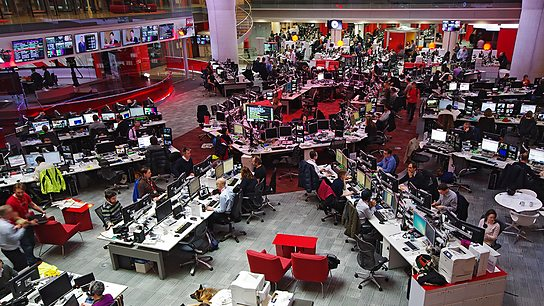
\includegraphics[width=\columnwidth]{figs/newsroom.jpg}
  \caption{The newsroom in BBC New Broadcasting House.}
  \label{fig:newsroom}
\end{figure}

Most of the work is based at a desktop PC and primarily done on the Electronic
News Production System (ENPS). This is an industry standard software package
for writing scripts and compiling news bulletins. It integrates with the
\textit{dira!} radio production system using a plugin called Media Object
Server (MOS). This allows users to browse and edit audio clips within ENPS (see
Section~\ref{sec:news-clips}).

\subsection{Workflow}
Each journalist produces one bulletin per hour, each between two and five
minutes long, depending on the network and the time of day (e.g. midday
bulletins are longer). Even if the stories being covered are the same, the
bulletins for each network are written separately so that they suit that
network's audience. This is done by varying the number of items, the amount of
detail and the level of assumed knowledge. The team aims to finish bulletins 15
mins before they are aired.

\subsubsection{Scripts}
Using ENPS, the team write text summaries of the current big news stories and
compile them into a bulletin. The information comes from a variety of sources,
but mainly from the news wires (e.g. Reuters) and BBC reporters.  The finished
bulletin must fit an exact time slot, so much of the work and skill is in
knowing how long the text will take to read and being able to condense the
story down to the key points. 

\subsubsection{Audio clips}\label{sec:news-clips}
Each bulletin contains a number of audio clips which help to break up the
newsreader's voice and make the piece more engaging.  Relevant audio content is
selected, edited to an appropriate length and inserted into the news script.
All clips are stored in \textit{dira!} and the MOS plugin is used to find, edit
and insert the clips into ENPS (see Figure~\ref{fig:news-enps-edit}).  This
uses \textit{dira!} Orion which offers basic cutting, levels and fading
functionality. When a clip is finished, it is dragged onto the script at the
point in the text where it should be played. The user must give the clip a
name, and can optionally add the in and out words\footnote{The 2/3 words spoken
  at the beginning and end of the recording.}. These and the clip duration
appear in the script which helps the journalists and newsreader.

\begin{figure}[ht]
  \centering
  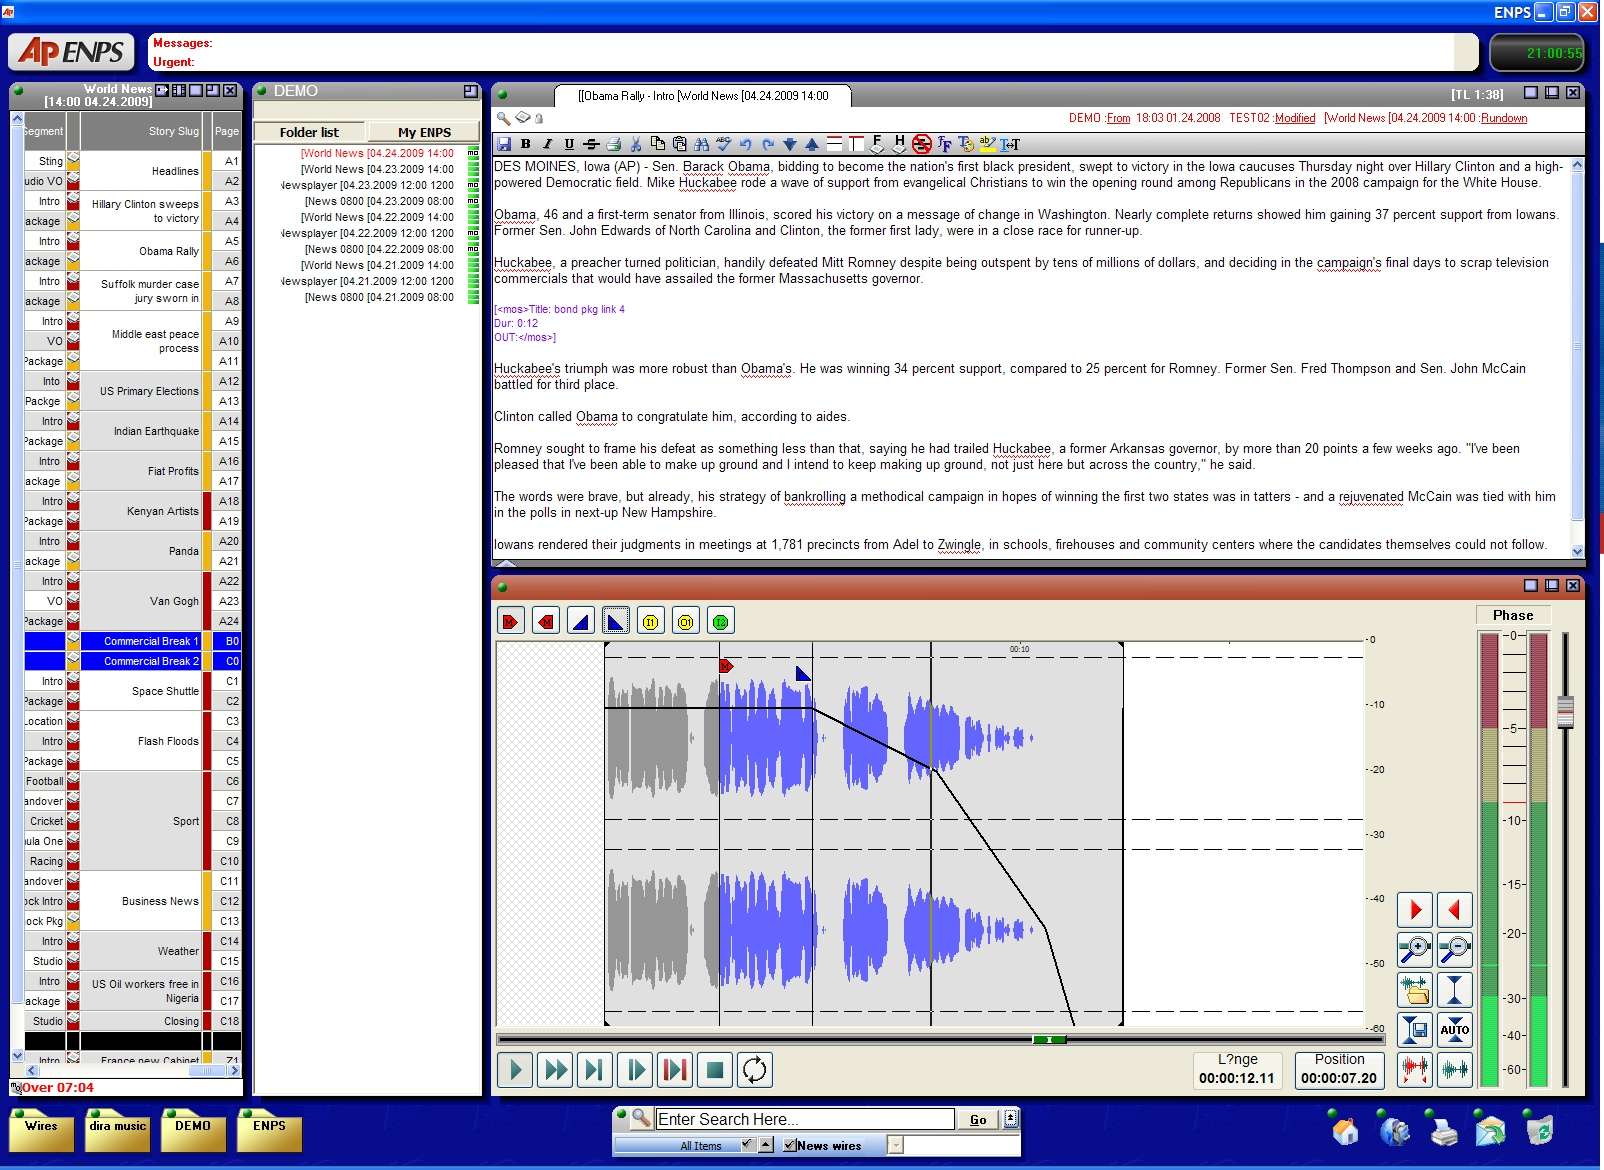
\includegraphics[width=\columnwidth]{figs/news-enps-edit.jpg}
  \caption{Editing a clip in ENPS using the MOS plugin for \textit{dira!}.}
  \label{fig:news-enps-edit}
\end{figure}

Audio content comes from a variety of sources including the intake team,
newswire team, and individual reporters (see Section~\ref{sec:news-roles}).
Off-air content from the BBC News TV channel is also used.  For off-air
recordings, the journalists must find and clip the audio themselves. Sound from
the TV channel is automatically recorded into \textit{dira!} in 40-minute
chunks. The recordings are navigated using the MOS plugin, which only displays
a waveform and timeline. Without knowing what time the clip starts, the
journalists resort to skipping through the 40 minutes listening out for a
familiar voice or word, which can be time-consuming and frustrating.

\subsubsection{Playout}
When a journalist has finished the scripts for their bulletin, these are placed
into a `running order' which is named with the network and time (e.g. `R4 Thu
10:00'). The assistant editor then reviews the scripts and listens to the clips
to ensure they comply with editorial policy and use the correct language and 
pronunciation.  Any required changes are made by the journalist or
editor before they are marked as approved. This gives the scripts a green label
in ENPS which indicates that they can be read on-air.

The presenter sits in a radio studio and normally has no direct contact with
the summaries team. At the time of the news bulletin, the presenter reads the
news scripts from ENPS live on-air. The audio clips in each script are
automatically loaded into the playout system, and the presenter triggers them
at the correct time.

\subsection{Challenges and opportunities}
Finding and cutting clips out of long recordings is a particular challenge.
There is very little information to go on so users resort to seeking through
the recording, listening out for someone's voice or mention of a certain topic.
The pressure of a fast turn-around makes the situation even more frustrating.
Application of segmentation or speech-to-text technology could help by
indicating where people are speaking, displaying keywords that are mentioned,
or allowing the recording to be searched by text.

When it comes to inserting clips into the script, in and out words are manually
entered so that the clip can be recognised, but there is not enough time to
transcribe the whole clip. Speech-to-text technology would be able to automate
this and full transcription could further help the journalists to recall the
clip and write the script around it.

\section{Drama}\label{sec:drama}
Radio 4's ``15 Minute Drama'' is a series of original drama and book
dramatisations, broadcast twice-daily. Production of radio drama is radically
different from that of news as it is based on a script of a radio play and is
created over a number of weeks.

\subsection{Roles}
The production team is made up of five members, plus a cast of actors. The
\textit{director} is the owner of the programme and works with the team to
create their interpretation of the radio play. The \textit{broadcast assistant}
handles the administrative side and during the recording, they annotate the
script with detailed notes. There are three \textit{studio managers} (SMs). The
\textit{panel SM} leads the recording process and operates the mixing desk.
The \textit{grams SM}\footnote{`Grams' refers to gramophones, originally the
  only way to play back sound effects.} makes the recordings and plays
pre-recorded sound effects.  The \textit{spot SM} works in the studio where
they place microphones and create spot effects\footnote{Known as `foley' in the
  movie industry.}.

\subsection{Environment}
The observed drama was recorded in studio 60A, which is a purpose-built
flexible performance space at BBC New Broadcasting House in London. It contains 
spaces with different acoustic properties including movable absorbers and a
foam-lined spiral corridor, used to simulate distance. There are many fixtures
and props for re-creating common environmental sounds including various
doors/windows, a staircase with both wood and carpet, a bedroom and a working
kitchen.

The studio is connected by a large acoustically-isolated window to the cubicle
where the production team sit (see Figure~\ref{fig:drama-studio}). The mixing
desk is in front of the window with the broadcast assistant to the right and
the director behind. The grams SM sits at the back of the room, while the spot
SM spends most of their time in the studio.

Post-production is done in an editing suite which is a compact
acoustically-treated room with a PC, speakers, small mixing desk and level
meters.

\begin{figure}[ht]
  \centering
  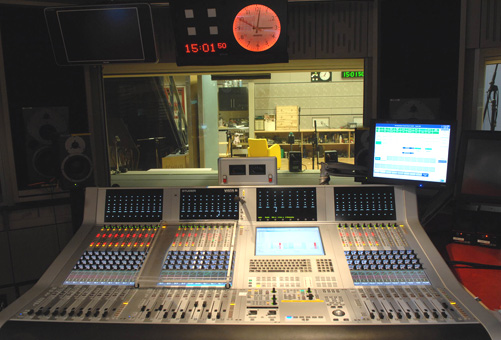
\includegraphics[width=\columnwidth]{figs/60a.jpg}
  \caption{Cubicle of studio 60A.}
  \label{fig:drama-studio}
\end{figure}

\subsection{Workflow}
Prior to the recording, the cast will have done a read-through where the
broadcast assistant notes the time taken to perform each scene.

\subsubsection{Recording}
The whole team is present during recordings and they normally record at least
one episode in a day. The scenes are done in sequence, with multiple takes
recorded for each. When the director is satisfied with the takes, the recording
moves onto the next scene.

During the recording, the panel SM balances the microphone feeds and sound
effects, and makes a backup recording onto a CD. The grams SM records the desk
output directly into a digital audio workstation (DAW) and stores each take as
a separate clip. The DAW is used to manually label each clip with the episode,
scene and take number (e.g. e2s3t1). The grams SM also selects and plays
environmental recordings and sound effects, which are recorded onto a separate
track in the DAW. The spot SM positions the microphones for the actors and
creates live spot effects in the studio. The director listens carefully to the
takes and makes their own notes.  Between takes, they discuss the performance
with the team and give feedback to the actors.

The broadcast assistant takes detailed notes throughout the recording by
annotating a paper copy of the script and keeping a spreadsheet of the takes
and their length. The paper annotations (see Figure~\ref{fig:drama-script})
have a well-defined syntax which is explained below. Although this syntax is
widely used, it is not formally defined so can vary from person-to-person.

A different coloured pen is used for each take. The start and end of each take
is marked with a vertical line on the side of the page, with the take and
backup CD numbers written at the top. If the take is repeated within a 
recording, the line continues back to the top. Repeated words or phrases are
marked with square brackets. If multiple brackets overlap, their order is
labelled with numbers.  Words that are spoken incorrectly are underlined. The
best take for each scene is marked by using highlighter pen on the vertical
line for that take.

\begin{figure}[p]
  \centering
  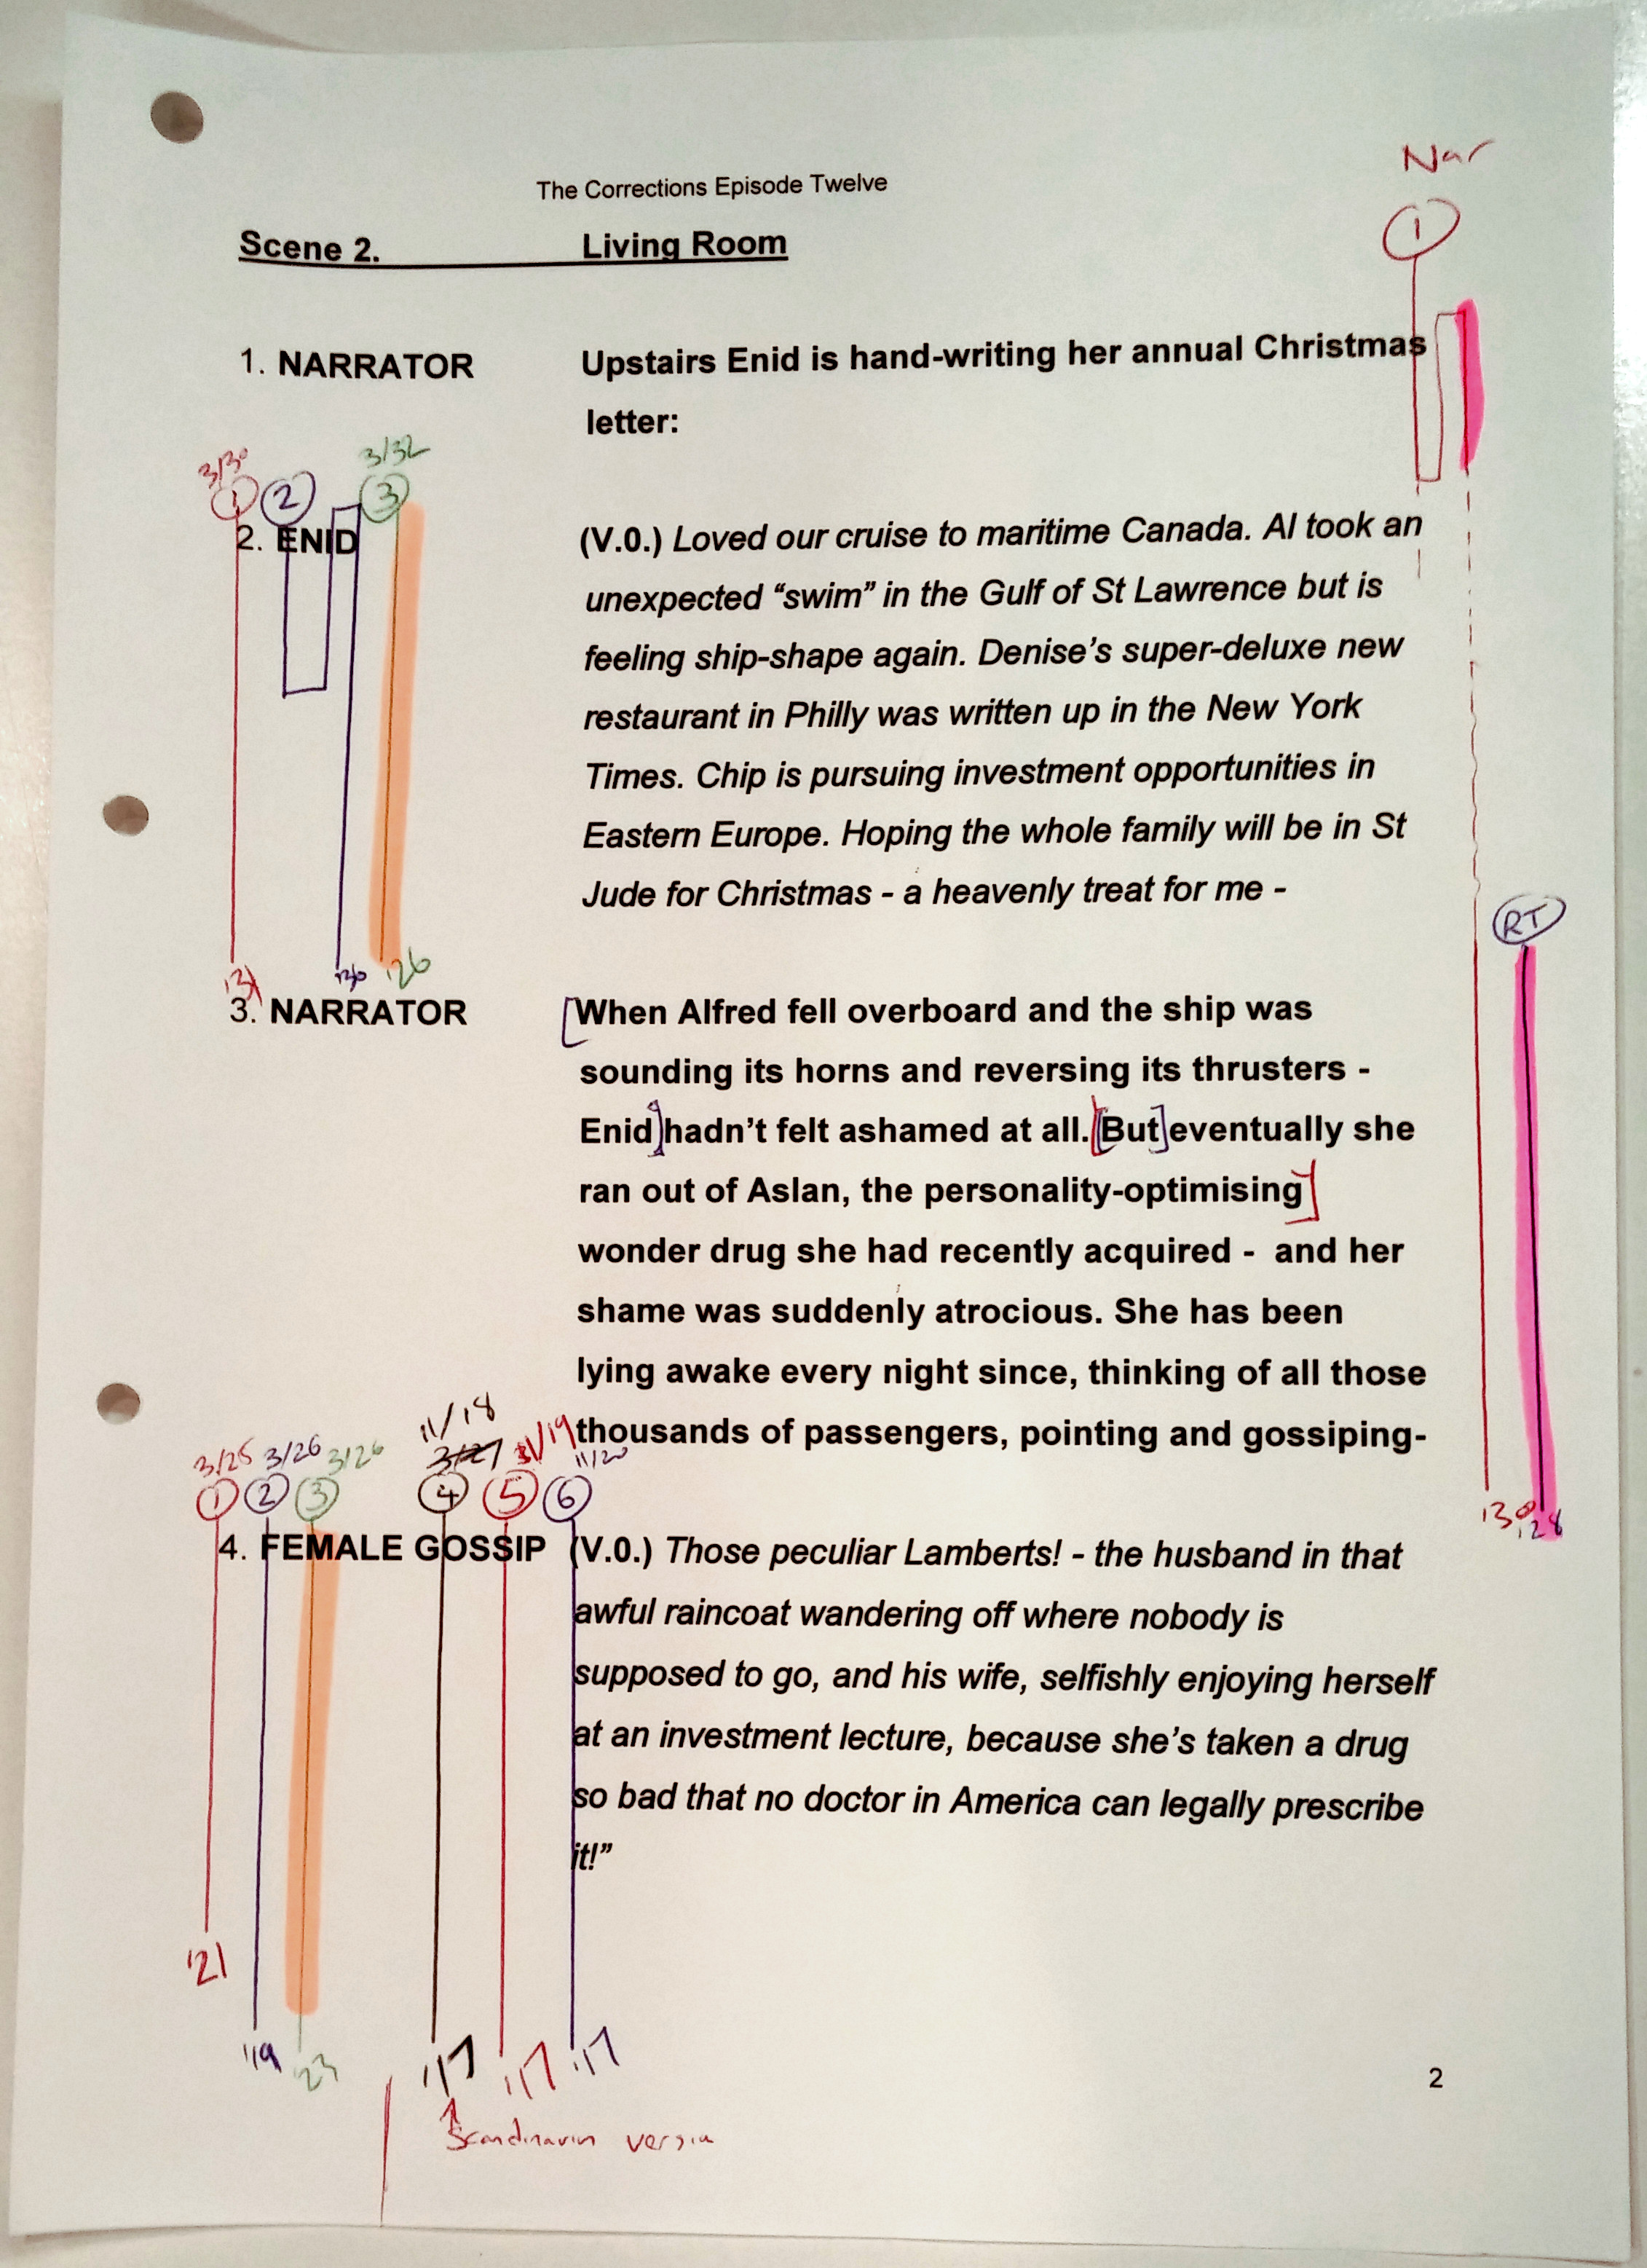
\includegraphics[width=\columnwidth]{figs/drama-script-example-processed.jpg}
  \caption{An annotated drama script page.}
  \label{fig:drama-script}
\end{figure}

After the recording is complete, the audio files are copied onto a portable
hard drive. Although hard drives can fail and be misplaced, they are still used
as the computer network is considered too slow and the hard drive can be taken
anywhere.

\subsubsection{Rough edit}
The rough edit is created with a DAW by one of the studio managers, usually the
panel SM. As the files are stored on a portable hard drive, this process can be
done either in an edit suite or on a laptop at home. The first step is to
create a sequence of the best takes from the recordings. The annotated script
is used to identify these, and they are dragged from the DAW's `clip list' onto
a timeline. There can be many clips, so sometimes they are searched with text
to narrow-down the list. Mislabelled clips or misread labels can occasionally
cause issues at this stage.

The script is used to identify and remove errors in the takes, particularly
re-takes or repeated words. Sometimes these are missed and must be removed
later. The sound level is adjusted to be consistent throughout, either by using
the mouse for in/out fades or by recording automation with a mixing desk
slider.

Sound effects that are listed in the script but were not played at the time of
recording are added at this stage. Roughly 600GB of effects are stored on the
local computer and their metadata can be searched using text. It takes skill
and experience to know which words to use for the search or to know which CDs
or collections to use for certain effects.

The recordings are listened to so that any unmarked errors are identified, such
as noise caused by actors handling the script during recording. Long sequences
are played at double-speed to save time.

\subsubsection{Fine edit}\label{sec:drama-fine}
Once the rough edit is complete, the director joins the SM in an edit suite to
cut the programme to the correct length, select the best performances, tweak
the sound effects and add background music.

The finished programme must have an exact duration to fill its assigned
broadcast slot. Almost always, the programme will be too long and some lines
must be removed. This can only be done by the director as these decisions have
a strong editorial impact.

While listening through the programme, the director may want to compare the
chosen take with other takes that were recorded. To do this, the SM must find
the correct recording using their labels, drag it onto the timeline and find
the right position in the recording. This process introduces an overhead which
can put directors off comparing performances too often.

Music is not specified in the script, so the director has the creative freedom
to choose what they want. Popular consumer music services are used to find
commercial tracks, but often directors will choose `production music', which is
designed for TV/radio and is easier to license. These are found using one of a
number of online music libraries which, similarly to the sound effects, are
searchable using descriptive keywords. The director provides the music to the
SM on a USB storage device for them to insert and mix.

Once finished, the final edit is mixed down to stereo by playing the programme
through a digital loop-back. Although this can be done automatically, it forces
the director and SM to listen to the programme from beginning to end in one
go.

\subsection{Challenges and opportunities}
The clear syntax used to annotate the drama script shows that the production
workflow is well-organised and makes good use of existing tools. However in the
rough edit stage, the SM is performing simple non-creative editing tasks based
purely on the annotations. If these could be captured in a digital format, the
rough edit stage could conceivably be fully or partly automated.

In addition to being script-based, a defining characteristic of drama
production is that multiple takes are recorded in order to capture the best
possible performance. However, there is no simple way to directly compare
performances so the director relies heavily on the script annotations and
written notes. Providing an easy method of comparing different takes by ear
could potentially lead to selection of better performances.

When actors fluff a line, they often say the line again immediately which is
usually noted in the script with square brackets. However, these can be missed
and are not easy to spot in a DAW. Simple audio analysis could be used to
detect and highlight where this happens.

\section{Documentary}\label{sec:doc}
``The Report'' is a weekly investigative documentary that covers topical news
stories. It is produced over a three week period by the BBC Current Affairs
team and is broadcast at 8pm every Thursday on Radio 4. The team was observed
for four days at various points during the three weeks.

\subsection{Roles}
The documentary is created by a core team of three people. The
\textit{producer} owns the programme. They decide what the story-line will be,
who to interview and how it is edited. The \textit{researcher} assists
the producer with research and investigation, setting up interviews and
transcribing recordings.  Both work full-time on the documentary throughout
the three weeks.  The \textit{presenter} is the narrator for the documentary.
The Report has a regular presenter who typically works on two or three
documentaries at once.

The team is supported by the \textit{editor} who runs the current affairs team.
They provide feedback on the documentary and must give approval for the
documentary to be broadcast. On the final day of production, a \textit{studio
  manager} (SM) joins the team to create the final edit.

\subsection{Environment}
The team is based in BBC New Broadcasting House in London. Their desks are
grouped together in an open-plan office, beside four studios. The studios are
organised into pairs so that one can be used for recordings and the other as a
control room. Each studio is acoustically treated and contains a PC, mixing
desk, microphones and a telephone.

\subsection{Workflow}
The three weeks it takes to create the programme can be very roughly divided
into research, interviews and editing. However in reality these activities
are dependent on external factors and can overlap significantly.

\subsubsection{Research}
The purpose of the research stage is to take the idea behind the programme and
form an interesting and relevant storyline around it. Often the topic will be
in the news that week, so the producer will be looking for an interesting angle
which can be explored in greater depth.

The research stage does not require any special tools other than a web browser
and a telephone. The team will read around the topic so that they are
knowledgeable enough to tell the story well and can identify a number of
people they want to interview. Popular sources of information are previous
reports or documentaries, newspaper articles, encyclopedias and contacts who
already know the subject. The producer will make rough notes for themselves in
Microsoft Word and prepare a draft outline of the programme.

\subsubsection{Interviews}
Once the team have identified who they would like to interview, they will
approach them to see if they are interested. If the interviewee has the time
available, the producer or researcher will do a `pre-interview' over the phone
to see what the person will say and whether it fits the documentary.

Most interviews are done face-to-face, either on-location or in a studio,
depending on the situation. A portable audio recorder and shotgun mic is used
for recordings outside of the studio. The presenter holds the microphone and
asks the questions while the producer controls the recorder and the microphone
level. Recordings in the studio are made straight into the \textit{dira!}
system using Orion.

If it's not possible to meet face-to-face, interviews can either be done using
a local studio and ISDN\footnote{Integrated Services Digital Network.  A
  communication standard that can be used to send low-latency digital audio
  over telephone networks.} link, over the phone but with a portable recorder
at each end\footnote{Known in the business as a `simulrec' or `mic hold'.},
using an IP-based link such as Skype, or just over the phone. The phone is
always a last resort as the quality is very poor.

\subsubsection{Rough edit}
When a producer is working on their own, they will usually edit the interviews
directly using a DAW. However, when a team is collaborating with 
interview material, all of the recordings are first transcribed. Some of
this is done using a third-party transcription service, but the programme's
budget can only cover transcription of three or four interviews. The rest must
be transcribed by the team themselves using Microsoft Word. Whereas the
professional transcription service includes every word, the team's own
transcriptions will skip out many words, leaving only enough to get a good idea
of what they said.

The transcriptions are printed out on paper and the team works with these
printouts until the last few days of production. Lines from the interviews that
they want to use in the programme are marked with highlighter pen. Other
informal notes are made on the paper.

The producer takes the annotated transcriptions and pieces together a rough
edit using \textit{dira!} StarTrack. As the position of each question in the
transcription is marked with a timestamp, the producer can narrow-down the
location of the highlighted text in the recording, but only to within a few
minutes. For each interview, the producer cuts out and saves any lines that
they have highlighted. These are then sequenced into a rough edit of the
programme.

While the producer creates the rough edit, the presenter writes the programme's
`links' -- the narrative elements that join the interview clips. When the first
rough edit is complete, the whole team sits down with the editor for a
`run-through'. The programme is performed out loud, straight-through from
beginning to end, with the presenter reading the links and the producer playing
the clips. This allows the editor to hear the programme and give feedback early
on, and for the length of the current edit to be determined. This run-through
process typically happens two or three times for each programme.

\subsubsection{Fine edit}
The fine edit happens on the day that the programme is to be broadcast. A
studio manager (SM) joins the team to create the final mix. The fine editing
requires that the rough edit is transferred into a DAW that has more features
than \textit{dira!} StarTrack.

The SM starts by cleaning up the interview clips. This is done by removing
redundant noises (e.g. `umm') and phrases (e.g. `you know'). Some are left in
as they are too difficult to remove or are editorially relevant. Long pauses
are removed to ensure there is a good pace, but are sometimes left in for
effect.  The SM also balances the levels by recording automation using a fader
or by dragging in/out fades. 

The links are recorded by the presenter who sits in the studio opposite the SM.
This is done straight into the DAW and the intro/outro to each clip is played
to the presenter. The producer sits in and gives feedback to the presenter over
an intercom. After the links are recorded, the SM goes back to correctly align
the interview and link clips in the timeline.

The Report has theme music which is added at this stage, along with any
additional music chosen by the producer. Similarly to drama (see
Section~\ref{sec:drama-fine}), production music is often used and is chosen
using an online library.

Once all of the elements have come together, the producer and SM must cut the
programme down to a specific duration (in this case 27:45). This is done by
removing sections of speech that can be cut without impacting on the story.
These are usually found at the beginning and end of interview clips.

The finished programme is played for the editor who gives their final feedback
and approval.  Once signed-off, the documentary is mixed down to a stereo .wav
file and imported into \textit{dira!}. The producer must then listen to the
entire programme in \textit{dira!} to ensure the bit-stream that will be
broadcast contains no errors.

\subsection{Challenges and opportunities}
The documentary production relies heavily on paper-based transcripts. This
allows the team to easily collaborate and to make notes, but means that there
is a disconnect between the words and audio content. This results in wasted
time when the producer has to go back and cut out the selected parts of the
interviews. There is also no easy way to listen back to a line in the
transcript. Creating a link between the transcripts and the audio recordings
would allow the producers to work with transcripts as normal, but to
simultaneously navigate and edit the audio content.

The fine edit revealed opportunities for assisting the studio manager with the
clean-up process. If an acoustic model of redundant noises and phrases was 
developed, these could either be highlighted, cut for easy removal or removed
automatically.

\section{Findings}\label{sec:summary}
Generally speaking, the study identified a number of opportunities to improve
the handling, generation and presentation of metadata, as discussed below.

\subsection{Text-based working}
The study found that the production teams relied strongly on scripts and
transcripts of the audio content. The rough edits for both the drama and
documentary were directly created from annotated scripts of the recordings.
Additionally, the news summaries team manually annotate their audio clips with
in/out words to help them identify the recordings. These workflows indicates
that producers would much rather work with text representations than with audio
on a timeline.

Creating a link between the words in the transcript and their position in the
audio could allow the producers to navigate and edit with text as they prefer,
but for the audio to be edited automatically. Hyperaudio \citep{Boas2012} is an
example of a web-based video editor that already uses this approach. In the
case of dramas and documentaries, the full text of the recordings is already
available so speech alignment technology such as SailAlign
\citep{Katsamanis2011} could be used instead of full speech-to-text.

\subsection{Use of paper}
Both the drama and documentary teams preferred to work with paper copies of the
scripts. Many producers are not technology-savvy and are therefore much more
comfortable with the idea of paper. It also affords them the freedom to make
unstructured notes and easily collaborate face-to-face. However, the use of
paper also creates a barrier between the work done on the page and the work
done on the screen. Digital pens and interactive paper are tools that have the
potential to break that barrier while retaining the advantages of both ways of
working. Further investigation is needed to see how such a system could
integrate the two approaches and whether the technology is viable.

\subsection{Redundant speech}
Observation of the fine edit in the documentary found that a significant
proportion of the studio manager's time was spent on cleaning-up interview
material. Much of this was caused by redundant noises such as `umm's and
`err's, or redundant phrases like `you know'. These could be identified using a
system designed or trained for the purpose.  Depending on the producer's
confidence in the algorithm, it could either remove the redundant material
automatically or assist the studio manager in identifying and removing the
material. 

\subsection{Speaker diarization}
All of the observed productions could benefit from being able to see where
different people are speaking in a recording, known as `speaker
diarization'. In drama it would help the producers identify different lines in
the script, in documentaries it would highlight the position of the questions
in interview recordings, and in news it would help producers find what they're
looking for more quickly in long off-air recordings. The research around
diarization is fairly mature \citep{AngueraMiro2012} and although it is starting
to be used in some experimental BBC services such as the World Service Archive
\citep{Raimond2014}, it has yet to become available any mainstream production
tools.

\subsection{Comparing takes}
Drama production is unique in the way it records multiple takes of the same
content. This technique allows the producers to get the most from the actors,
but means that it can be difficult to select which performances to use.
Comparing takes during post-production is possible but the process is clumsy.
Providing an easy way to directly compare performances would allow the director
to make a better informed decision on which to use. If the rough edit for the
drama was assembled automatically, comparison could be made easier by aligning
the takes on different tracks.

\section{Conclusion}\label{sec:conclusion}
An ethnographic study of radio production was conducted by exploring three case
studies. It found that producers of speech radio prefer to work with text-based
representations of audio rather than with the recordings directly. Their
workflows are primarily paper-based which creates extra work when moving
between paper and audio. Creating a link between the words on the paper and
their location in the audio recordings could significantly improve the
production workflow.

The study also identified opportunities to apply semantic audio technology and
interaction design to radio production tasks. Lots of time is spent cleaning up
recordings by removing redundant speech, which could be fully or
semi-automated. Segmenting speech content by speaker would make a positive
impact on most speech-based tasks. Finally, drama productions could benefit
from an easy way to compare multiple takes of the same scenes.
